\begin{coverpage}{Introduction}
{
Welcome to the second workshop of Single Cell \& Spatial Omics Korea (SCSOK), a platform where researchers in Korea converge to explore and share their insights in the rapidly evolving fields of single-cell and spatial omics. This abstract book serves as a guide and a record of the pioneering research and collaborative efforts showcased in our workshop.

\subsubsection*{Our Community: Uniting Diverse Expertise in Various Backgrounds}
SCSOK is an open community of researchers with varied backgrounds in biology, medicine, computer science, mathematics, engineering, and statistics. We are wet-lab and dry-lab researchers interested in developing novel methods and/or applying them in the field of single-cell and spatial omics. Our diversity is our strength, fostering a rich interdisciplinary collaboration and innovation environment.

\subsubsection*{Our Vision: Advancing Single-cell and Spatial Omics Research}
Our mission is to advance the study of single-cell and spatial omics, pushing the frontiers of knowledge and application. In addition to the workshop, we plan to host many more exciting events, for example, data hackathons and an online lecture series. These plans are aimed at fostering collaboration, innovation, and knowledge exchange among researchers in Korea and contributing to global progress in these fields.

\subsubsection*{Our Progress: A Brief History of SCSOK}
SCSOK has rapidly grown since its inception, marking several significant milestones:

\begin{itemize}[leftmargin=0.5cm, rightmargin=0.5cm]
\item January 4-5, 2023: Our first workshop on single-cell and spatial omics at the Institute for Basic Science in Daejeon, co-organized by Drs. Bon-Kyoung Koo, Jeongbin Park, and Junil Kim.
\begin{figure}[h!]
\vspace{3mm}
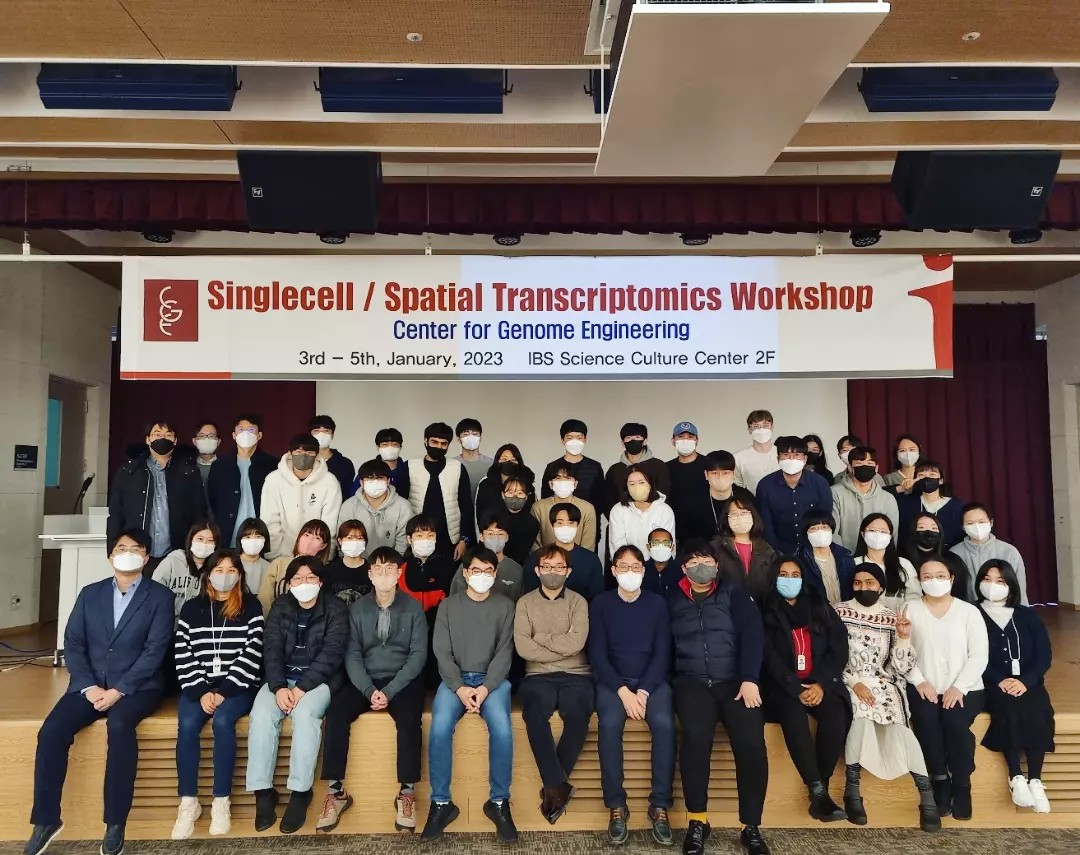
\includegraphics[width=\textwidth]{images/1st-workshop.jpg}
\centering
\end{figure}
\item January 6, 2023: Set up Zulip as a means of communication, following the first successful workshop.
\item October 26, 2023: Agreement on having the second workshop in Yangsan, co-organized by Drs. Jeongbin Park, Junil Kim, and Heetak Lee.
\item October 27, 2023: Acquisition of the \textbf{\texttt{scsok.io}} domain, establishing our online presence.
\item October 27-29, 2023: Development the \textbf{\texttt{scsok.io}} website, a hub for ongoing updates and resources.
\item November 1, 2023: Kickoff meeting for the upcoming workshop.
\item November 1-16, 2023: Invitation of domestic and international speakers.
\item January 22-23, 2024: The second single-cell \& spatial omics workshop.
\end{itemize}

This book contains the abstracts of presentations and posters from our esteemed participants. Each abstract represents a unique contribution to the field, offering insights into the latest research, methodologies, and findings in single-cell and spatial omics.
\\
\subsubsection*{Looking Forward: Building a Stronger Community}
As you explore this abstract book, we encourage you to engage with the ideas and connect with fellow researchers. This workshop is not just an event; it's a step towards building a stronger, more collaborative scientific community in Korea.
\\
\\
\textbf{Welcome to the 2nd SCSOK Workshop. Together, let's explore the depths of single-cell and spatial omics and shape the future of scientific discovery.}
\\
\vspace{1cm}
\\
\noindent
Best regards, \\ Workshop Organizing Committee \\ Jeongbin Park, Junil Kim, Heetak Lee
}
\end{coverpage}